\section{Related Work}
\label{sec:related}

\paragraph{3D Object Detection:}

We can categorize 3D detectors by their input modality (e.g., LiDAR, camera), scene representation (e.g., point clouds, voxels), and number of stages (e.g., single-stage or multi-stage)

LiDAR-based methods commonly represent the input as
voxels~\cite{yan2018second,hednet,safdnet,li20173d,engelcke2017vote3deep,song2016deep}, pillars~\cite{ku2018joint,lang2019pointpillars,simony2018complex,wang2015voting,wang2020pillar,yang2018pixor},
or point clouds~\cite{ngiam2019starnet,wu2024point,shi2019pointrcnn,shi2020point,yang20203dssd}.
A widely used approach for including temporal LiDAR information is \textit{point aggregation}, which involves
transforming past point clouds into a common coordinate frame and processing the aggregated point cloud.
These approaches are usually limited to $\le 5$ past LiDAR frames due to computational constraints~\cite{li2023modar} in online applications like autonomous driving.
Another drawback is that point aggregation does not align moving objects, requiring a larger receptive field in the detector backbone the longer the temporal horizon is~\cite{safdnet,li2023modar}.

Camera-based 3D detection is challenging because of missing depth information.
One approach is to produce 3D bounding boxes from image features
by estimating depth, 3D size, and orientation~\cite{wang2021fcos3d,xu2018multi,chen20153d,mousavian20173d}.
Other methods leverage voxel~\cite{roddick2018orthographic,reading2021categorical,qian2020end} or point cloud~\cite{wang2019pseudo,you2019pseudo} representations
by predicting pixel depth distributions to lift 2D features to 3D.
Stacking and processing past camera images or feature maps
is a common but expensive method for temporal fusion~\cite{zeng2022lift,piergiovanni20214d,hu2021fiery,saha2022translating,can2022understanding}.

Regardless of modality, we can further categorize 3D detectors as single-stage or multi-stage. Single-stage methods produce detections from sensor data~\cite{safdnet,hednet,yan2018second,engelcke2017vote3deep,wang2021fcos3d,chang2024bevmap} with a single deep neural network.
Multi-stage methods use bounding box proposals from a first stage (or randomly initialized proposals)
to gather features (e.g., with RoIPool~\cite{ren2015faster}, RoIAlign~\cite{he2017mask},
interpolations~\cite{centerpoint}, or attention~\cite{zhou2022centerformer,casas2024detra,li2023dfa3d,lin2022sparse4d,wang2022detr3d,liu2022petr,liu2023petrv2})
and iteratively refine the bounding boxes.

\ourmodel{} is a sensor-modality-agnostic module that we can add to any detector as a subsequent refinement stage.
In our work we utilize CenterPoint~\cite{centerpoint}, SAFDNet~\cite{safdnet}, HEDNet~\cite{hednet}, FCOS3D~\cite{wang2021fcos3d}, and BEVMap~\cite{chang2024bevmap} as proposal networks.

\paragraph{Long-Term Temporal Fusion for 3D Detection:}

Various works attempt to solve the shortcomings of sensor aggregation by learning to use multiple seconds of sensor evidence to improve object detection.

In this line of work, the \textit{scene-based} paradigm uses
recurrent fusion of scene-level features~\cite{frossard2021strobe,he2023lef,li2022bevformer,centerpoint},
with some methods relying on multiple traversals of the scene~\cite{you2022hindsight}.
A challenge of this approach is focusing and aligning features from relevant and dynamic foreground objects,
which past works addressed by transforming feature maps, using segmentation to focus on foreground objects~\cite{he2023lef},
and using deformable attention or convolution to align features of moving objects~\cite{koh2023mgtanet}.
Processing both foreground and background areas can be computationally expensive.
It is worth noting that many of these methods are single-stage detectors~\cite{frossard2021strobe,he2023lef} and which we could use as a detection proposal network with \ourmodel{}.

\begin{figure*}[t]
    \centering
    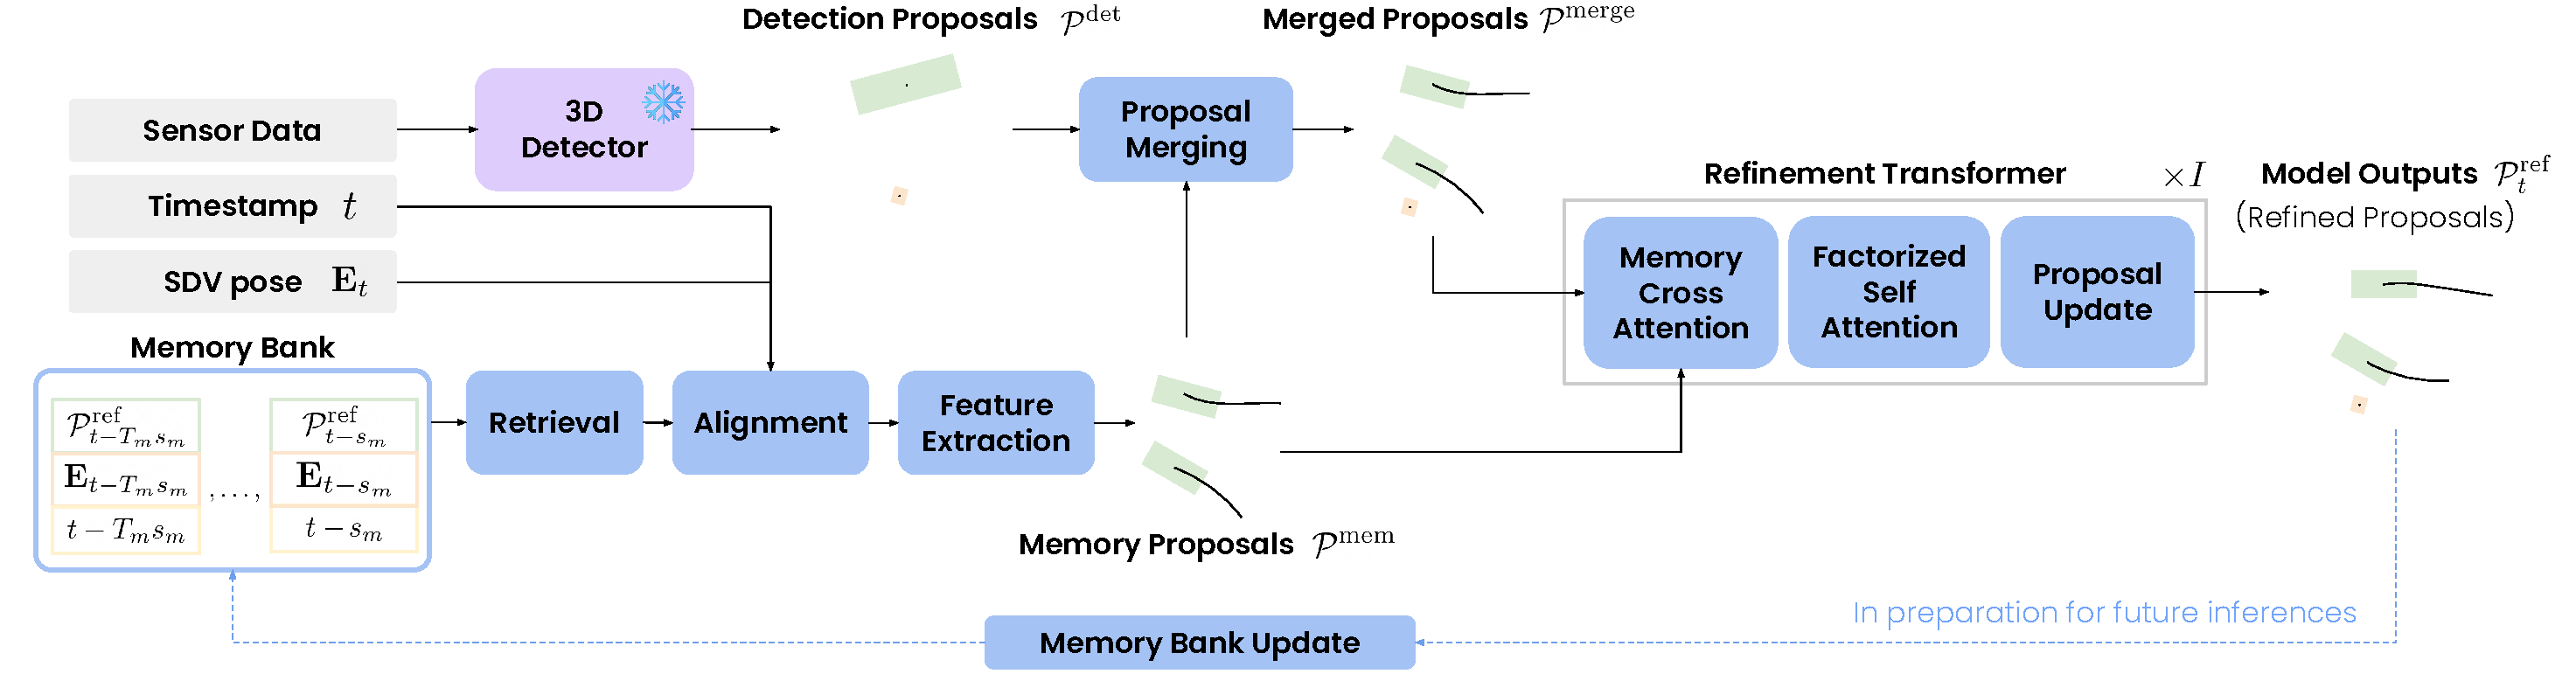
\includegraphics[width=\textwidth]{images/architecture_v7.pdf}
    \caption{
        \ourmodel{} is a plug-and-play module that enhances any off-the-shelf 3D detector (kept frozen) with long-term memory. 
        }
    \vspace{-5mm}
    \label{fig:arch}
\end{figure*}

Alternatively, the \textit{object-based} paradigm focuses on
the foreground by using detection proposals.
\textit{Detect-track-fuse} methods are a sub-family of object-based methods that associate previous detections over time to create tracks,
and these tracks summarize information from past sensor evidence
~\cite{liang2020pnpnet,huang2024ptt,chen2022mppnet,li2023modar,zhang2023motiontrack,li2023modar}.
However, in complex situations like pedestrian crowds, association over time can be difficult due to heavy occlusions and erratic behavior, potentially leading to false negatives or identity switches in the tracks.
\textit{Object-to-scene} approaches mitigate the shortcomings of association by directly using current detection proposals to aggregate historical scene-level information using hand-crafted feature aggregation modules~\cite{he2023msf} or attention mechanisms~\cite{zhou2022centerformer}.
These approaches can be difficult to scale to long history horizons as they require re-processing past sensor evidence or dense feature maps based on the current proposals
(e.g., \cite{zhou2022centerformer,he2023msf} only use 0.7s of history).
Finally, \textit{object-to-object} methods
use past object detections to improve current object detections without explicit tracking,
e.g., by cross-attending from current detection proposals to past detections~\cite{yang20213d,wang2023exploring},
or using hand-coded attention matrices based on distance~\cite{hou2024query}.
Overall, most object-based methods share some deficiencies:
Many only refine detection proposals produced by current sensor evidence and struggle to recover from missing proposals~\cite{he2023msf,yang20213d,hou2024query,chen2022mppnet,huang2024ptt}.
Others naively concatenate past detections with current proposals~\cite{wang2023exploring}, which
can lead to alignment issues for dynamic objects and miss-calibration in the proposal scores, as the model should trust historical proposals less than current proposals.

Our proposed method, \ourmodel{}, performs object-based temporal fusion without requiring explicit object association, aligns the memory in space and time by with trajectory forecasting,
and can recover from missing proposals by using and rescoring proposals from the memory bank.